% This is samplepaper.tex, a sample chapter demonstrating the
% LLNCS macro package for Springer Computer Science proceedings;
% Version 2.20 of 2017/10/04
%
\documentclass[runningheads]{llncs}
%%%%%
\usepackage{eqnarray,amsmath}
\usepackage{subfig}
\usepackage{graphicx}
\usepackage{amsfonts}
\usepackage{amssymb}
% Used for displaying a sample figure. If possible, figure files should
% be included in EPS format.
%
% If you use the hyperref package, please uncomment the following line
% to display URLs in blue roman font according to Springer's eBook style:
% \renewcommand\UrlFont{\color{blue}\rmfamily}
\setlength{\textfloatsep}{4pt plus 1.0pt minus 1.5pt}
\setlength{\floatsep}{4pt plus 1.0pt minus 1.5pt}

\begin{document}
\setlength{\abovedisplayskip}{3pt}
\setlength{\belowdisplayskip}{3pt}
%
\title{Comparison of dimensionality reduction schemes for parallel global optimization
algorithms
\thanks{The study was supported by the Russian Science Foundation, project No 16-11-
10150}}
%
\titlerunning{Dimension reduction schemes in parallel GO}
% If the paper title is too long for the running head, you can set
% an abbreviated paper title here
%
\author{Konstantin Barkalov \and
Vladislav Sovrasov \and
Ilya Lebedev}
%
\authorrunning{K. Barkalov et al.}
% First names are abbreviated in the running head.
% If there are more than two authors, 'et al.' is used.
%
\institute{
Lobachevsky State University of Nizhni Novgorod, Nizhni Novgorod, Russia
\email{konstantin.barkalov@itmm.unn.ru}\\
\email{sovrasov.vlad@gmail.com}\\
\email{ilya.lebedev@itmm.unn.ru}\\
\url{http://hpc-education.unn.ru/}
}
%
\maketitle              % typeset the header of the contribution
%
\begin{abstract}
This work considers a parallel algorithms for solving multi-extremal optimization problems.
Algorithms are developed within the framework of the information-statistical approach and
implemented in a parallel solver Globalizer. The optimization problem is solved by reducing
the multidimensional problem to a set of joint one-dimensional problems that are solved in
parallel. Five types of Peano-type space-filling curves are employed to reduce dimension. The
results of computational experiments carried out on several hundred test problems are discussed.

\keywords{Global optimization \and  Dimension reduction \and Parallel algorithms  \and
Multidimensional multiextremal optimization  \and Global search algorithms  \and Parallel
computations }
\end{abstract}

%------------------------------------------------------------------------------
\section{Introduction}\label{sec:intro}
%\begin{Russian}

In the present paper, the parallel algorithms for solving the multiextremal optimization problems
are considered. In the multiextremal problems, the opportunity of reliable estimate of the global
optimum is based principally on the availability of some information on the function known
{\textit a priori} allowing relating the probable values of the optimized function to the known
values at the points of performed trials. Very often, such an information on the problem being
solved is represented in the form of suggestion that the objective function $\varphi(y)$ satisfies
Lipschitz condition with the constant $L$ not known a priori (see, for example,
\cite{Jones,Gablonsky,Evtushenko}). At that, the objective function could be defined by a
program code i. e. could represent a ``black-box''-function. Such problems are presented in the
applications widely (problems of optimal design of objects and technological processes in
various fields of technology, problems of model fitting according to observed data in scientific
research, etc.).

Many methods destined to solving the problems of the class specified above reduce the solving
of a multidimensional problem to solving the one-dimensional subproblems implicitly (see, for
example, the methods of diagonal partitions \cite{SergeyevKvasov2015} or
simplicial partitions \cite{Zilinskas2014}). In the present work, we will use the
approach developed in Lobachevsky State University of Nizhni Novgorod based on the idea of
the dimensionality reduction with the use of Peano space-filling curves $y(x)$ mapping the
interval $[0,1]$ of the real axis onto an $n$-dimensional cube continuously and unambiguously.

Several methods of constructing the evolvents approximating the theoretical Peano curve have
been proposed in \cite{strongin1978,Strongin1992,Goryachih2017,Gergel2009}. These
methods were implemented in the Globalizer software system \cite{globalizerSystem}. The goal
of the present study was comparing the properties of the evolvents and the selecting the most
suitable ones for the use in the parallel global optimization algorithms.

%\end{Russian}
%------------------------------------------------------------------------------
\section{Statement of Multidimensional Global Optimization Problem}
In this paper, the core class of optimization problems, which can be solved using
Globalizer, is formulated. This class involves the multidimensional global
optimization problems without constraints, which can be defined in the following way:
\begin{equation}
\label{eq:task}
\begin{array}{cr}\\
  \varphi(y^*)=\min\{\varphi(y):y\in D\}, \\
  D=\{y\in \mathbb{R}^N:a_i\leq y_i\leq{b_i}, 1\leq{i}\leq{N}\}
\end{array}
\end{equation}
with the given boundary vectors  $a$ and  $b$. It is supposed, that the objective function
\(\varphi(y)\) satisfies the Lipschitz condition
\begin{equation}
\label{eq:lip}
|\varphi(y_1)-\varphi(y_2)|\leq L\Vert y_1-y_2\Vert,y_1,y_2\in D,
\end{equation}
where \(L>0\) is the Lipschitz constant, and \(||\cdot||\) denotes the norm in \(\mathbb{R}^N\)
space.
\par
Usually, the objective function \(\varphi(y)\) is defined as a computational procedure,
according to which the value \(\varphi(y)\) can be calculated for any vector \(y\in D\)
(let us further call such a calculation \textit{a trial}). It is supposed that this procedure
is time-consuming.
%As a result, the overall time of solving the optimization
%problem (\ref{eq:task}) is determined, first of all by the number of executed trials.
%It should also be noted that the requirement of the Lipschitz condition (\ref{eq:lip})
%is highly important, since an estimate of the global minimum can be constructed on the
%basis of a finite number of computed values of the optimized function only in this case .

%------------------------------------------------------------------------------
\section{Methods of Dimension Reduction}
\subsection{Single evolvent}

Within the framework of the information-statistical global optimization theory,
the Peano space-filling curves (or evolvents) \(y(x)\) mapping the interval \([0,1]\)
onto an \(N\)-dimensional hypercube \(D\) unambiguously are used for the dimensionality
reduction \cite{sergeyevStronginLera2013}, \cite{strongin1978},
\cite{stronginGergelBarkalovParGO}, \cite{strSergGO}.
\par
As a result of the reduction, the initial multidimensional global optimization
problem (\ref{eq:task}) is reduced to the following one-dimensional problem:
\begin{equation}
\label{eq:oneDimTask}
\varphi(y(x^*))=\min\{\varphi(y(x)):x\in [0,1]\}.
\end{equation}
\par
It is important to note that this dimensionality reduction scheme transforms the % minimized
Lipschitzian function from (\ref{eq:task}) to the corresponding one-dimensional
function \(\varphi(y(x))\), which satisfies the uniform H{\"o}lder condition, i. e.
\begin{equation}
\label{eq:holder}
|\varphi(y(x_1))-\varphi(y(x_2))|\leq H{|x_1-x_2|}^{\frac{1}{N}}, x_1,x_2\in[0,1],
\end{equation}
where the constant $H$ is defined by the relation \(H=2L\sqrt{N+3}\), \(L\) is the Lipschitz
constant from (\ref{eq:lip}), and \(N\) is the dimensionality of the optimization problem
(\ref{eq:task}).
\par
The algorithms for the numerical construction of the Peano curve approximations are
given in \cite{strSergGO}.

\par
The computational scheme obtained as a result of the dimensionality reduction consists of the
following:
\begin{itemize}
  \item The optimization algorithm performs the minimization of the reduced one-dimensional
  function \(\varphi(y(x))\) from (\ref{eq:oneDimTask}),
  \item After determining the next trial point \(x\), a multidimensional image \(y\) is calculated by
using the mapping \(y(x)\),
  \item The value of the initial multidimensional function \(\varphi(y)\) is calculated at the point
\(y\in D\),
  \item The calculated value \(z=\varphi(y)\) is used further as the value of the reduced one-dimensional function \(\varphi(y(x))\) at the point \(x\).
\end{itemize}

%------------------------------------------------------------------------------
\subsection{Shifted evolvents}
\label{sec:shifted}

One of the possible ways to overcome the negative effects of using a numerical
approximation of evolvent (it destroys the information about the neighbor points in $\mathbb{R}^N$ space,
see \cite{Strongin1992}) consists in using the multiple mappings
\begin{equation}%\label{eq:142}
Y_L(x)=\left\{y^0(x),\ y^1(x),...,\ y^L(x)\right\}
\end{equation}
instead of single Peano curve $y(x)$ (see \cite{Strongin1992,strSergGO,Strongin1991}).

Such set of evolvents can be produced by shifting the source evolvent $y^0(x)$ by $2^{-l},0
\leq l \leq L$ on each coordinate. Each evolvent has it's own corresponding hypercube $D_l=
\left\{y \in R^N: -2^{-1} \leq y_i+2^{-l} \leq 3 \cdot 2^{-1},\ 1\leq i\leq N\right\},\ 0 \leq l \leq
L$.

In Fig.~\ref{fig:shifted_ev} the image of the interval $[0,1]$ obtained by the curve $y^0(x),\
x\in [0,1],$ is shown as the dashed line. Since the hypercube $D$ from (\ref{eq:task}) is
included in the common part of the family of hypercubes $D_l$, having introduced an additional constraint
function
\begin{equation}\label{6_g0}
g_0(y)=\max\left\{\left|y_i\right| - 2^{-1}:\ 1\leq i\leq N\right\},
\end{equation}
one can present the initial hypercube $D$ in the form
\[
D=\left\{y^l(x):\; x\in [0,1],\ g_0(y^l(x))\leq 0 \right\},\ 0\leq l \leq L,
\]
i.e., $g_0(y) \leq 0$ if $y\in D$ and $g_0(y)>0$ otherwise. Consequently, any point $y \in D$
has its own preimage $x^l \in [0,1]$ for each mapping $y^l(x),\ 0\leq l\leq L$.

Thus, each evolvent $y^l(x),\ 0\leq l \leq L,$ generates its own problem of the type
(\ref{eq:task}) featured by its own extended (in comparison with $D$) search domain $D_l$
and the additional constraint with the left hand part from (\ref{6_g0})
\begin{equation}\label{6_problem_l}
\min{\left\{\varphi(y^l(x)):x\in [0,1], \; g_j(y^l(x))\leq 0, \; 0 \leq j \leq m\right\}}, \ 0 \leq l \leq L.
\end{equation}

\begin{figure}[ht]
    \centering
    \subfloat[Two shifted evolvents on the hypercubes $D_0$ and $D_1$]{{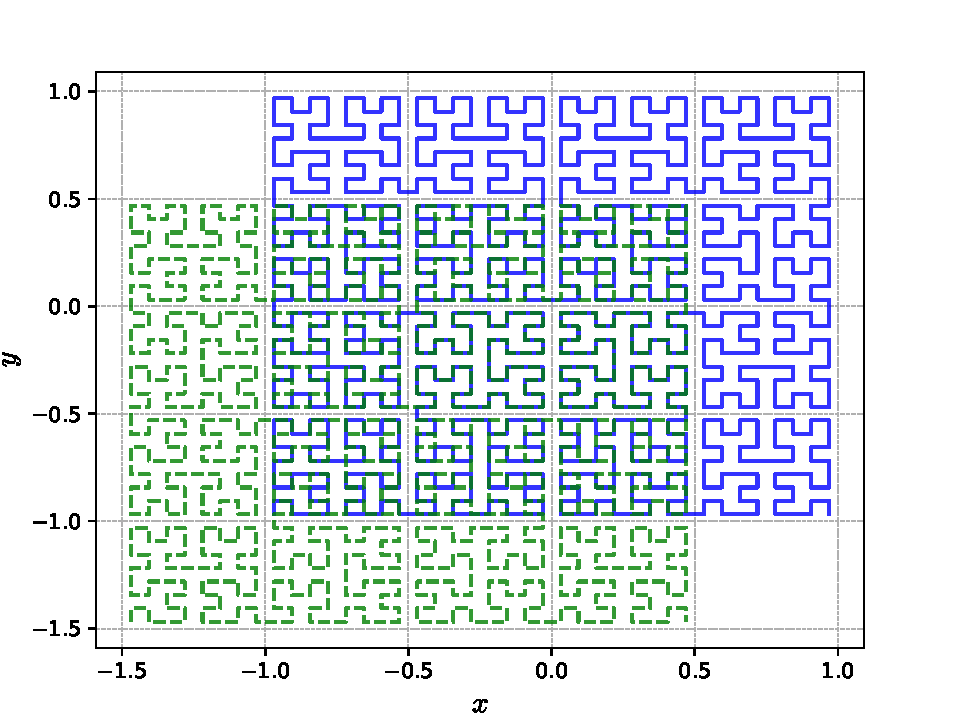
\includegraphics[width=.5\textwidth]{pictures/shifted.pdf}}\label{fig:shifted_ev}}
    %\subfloat[Hypercubes $D_l$]{{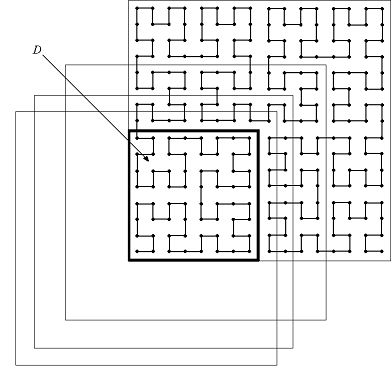
\includegraphics[width=.4\textwidth]{pictures/shifted_cube.png}}\label{fig:shifted_cube}}
    \subfloat[Two rotated evolvents on the same plane]{{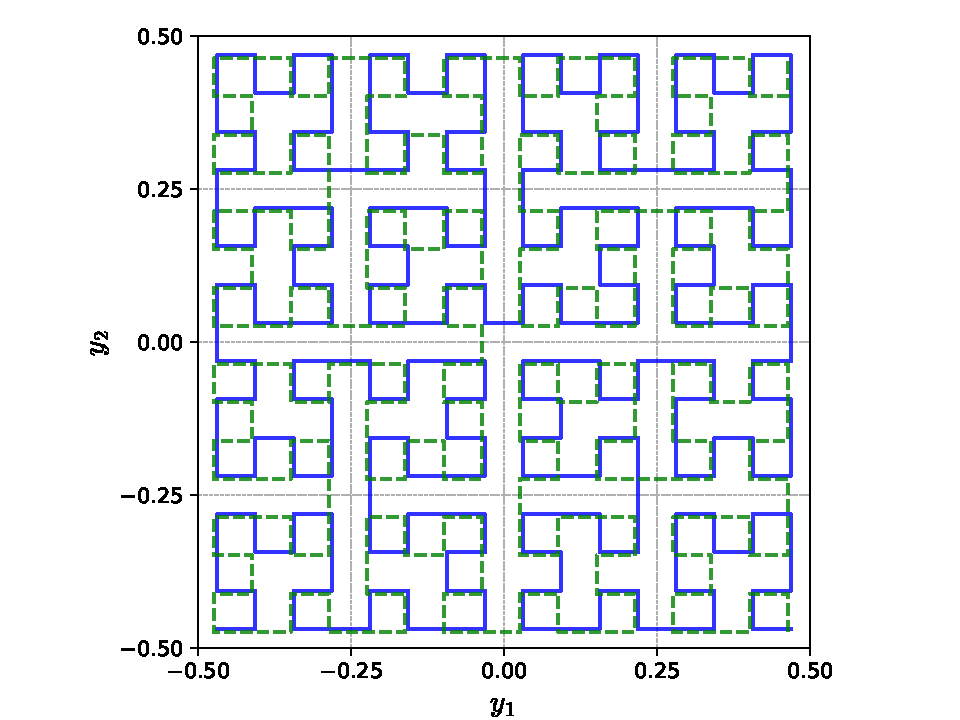
\includegraphics[width=.5\textwidth]{pictures/rotated.pdf}}\label{6_fig_9}}
    \caption{Multiple evolvents built with low density }
\end{figure}

%------------------------------------------------------------------------------
\subsection{Rotated evolvents}
The application of the scheme for building the multiple evolvents (hereinafter called the shifted
evolvents or $S$-evolvents) described in Subsection \ref{sec:shifted} allows to preserve the
information on the nearness of the points in the multidimensional space and, therefore, to
provide more precise (as compared to a single evolvent) estimate of Lipschitz constant in the
search process. However, this approach has serious restrictions, which narrow the applicability
of the parallel algorithms, designed on the base of the $S$-evolvents (see the end of the section
\ref{sec:seq_comp}).

To overcome complexity of the $S$-evolvent and to preserve the information on the nearness of the points in
the $N$-dimensional space, one more scheme of building of the multiple mappings was proposed.
The building of a set of Peano curves not by the shift along the main diagonal of the hypercube
but by rotation of the evolvents around the coordinate origin is a distinctive feature of the
proposed scheme \cite{Gergel2009}.
In Fig.~\ref{6_fig_9} two evolvents being the approximations to Peano curves for the case
$N=2$ are presented as an illustration.
Taking into account the initial mapping, one can conclude that current implementation of the
method allows to build up to $N(N-1)+1$ evolvents for mapping the $N$-dimensional domain
onto the corresponding one-dimensional intervals. Moreover, the additional constraint  $g_0(y)
\leq 0$ with $g_0(y)$ from (\ref{6_g0}), which arises in shifted evolvents, is absent. This
method for building a set of mappings can be ``scaled'' easily to obtain more evolvents (up to
$2^N$) if necessary.

%\begin{figure}[t]
%  \centering
%  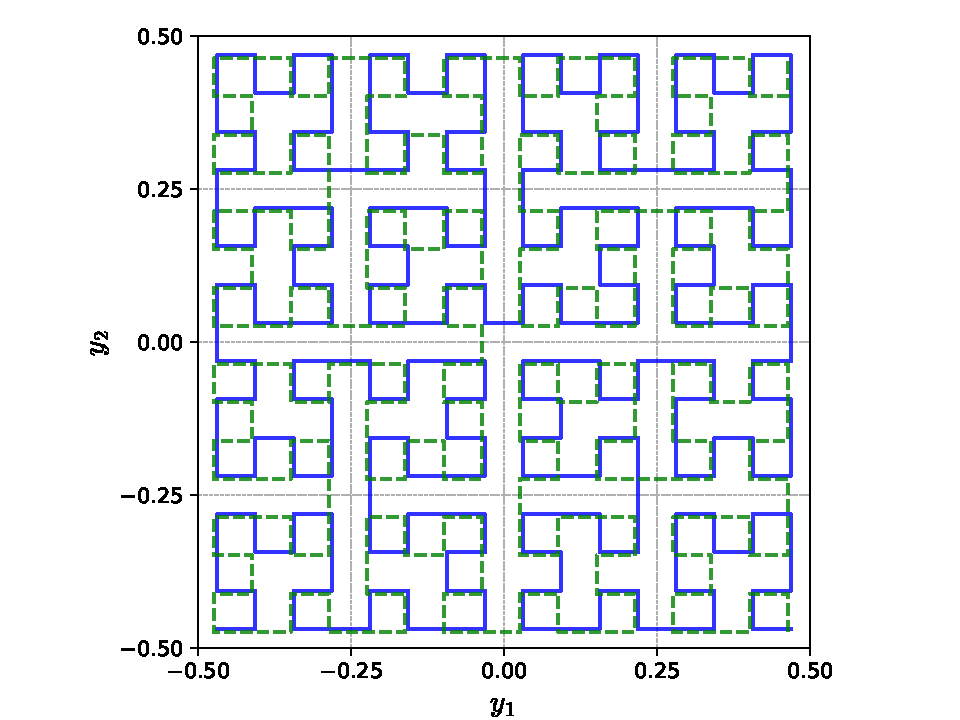
\includegraphics[width=0.6\linewidth]{pictures/rotated.pdf}
%  \caption{Two rotated evolvents on the same plane}
%  \label{6_fig_9}
%\end{figure}

%------------------------------------------------------------------------------
\subsection{Non-Univalent evolvent}
%\begin{Russian}

As it has been already mentioned above (Sec.~\ref{sec:shifted}), the loss of information on the
proximity of the points in the multidimensional space could be compensated in part by the use
of multiple mappings $Y_L(x)=\{y^1(x),...,y^L(x)\}$. However, the Peano-type curve preserves
a part of this information itself: it is not an injective mapping. Therefore, if a single image
$y(x)\in \mathbb{R}^N$ is available, one can obtain several different preimages
$t_j\in[0,1], t_j \not = x$, which could be added into the search information of the method later.

The Peano-type curve used in (\ref{eq:oneDimTask}) for the dimensionality reduction is
defined via the transition to the limit. Therefore, it cannot be computed directly. In the
numerical optimization, some approximation of this curve is used, and it is an injective piecewise-linear curve. In \cite{strongin1978} a non-univalent mapping of a uniform grid in the
interval $[0,1]$ onto a uniform grid in a hypercube $D$ has been proposed. Each
multidimensional node can have up to $2^N$ one-dimensional preimages. In
Fig.~\ref{fig:noninjective}, the grid in the $\mathbb{R}^2$ space is marked by the crosses, for
two nodes of which the corresponding one-dimensional preimages from $[0,1]$ are pointed
(marked by the squares and circles). Each node mentioned above has 3 preimages.

A potentially large number of preimages (up to $2^N$) and the inability to use the parallel
scheme for the multiple mappings form Sec.~\ref{sec:parallel_evolvents} are the disadvantages
of the non-univalent evolvent.


%------------------------------------------------------------------------------
\subsection{Smooth evolvent}

The methods of constructing the evolvents considered in the previous paragraphs produce the
curve $y(x)$, which in not a smooth one (see Fig.~\ref{fig:shifted_ev}). The absence of
smoothness may affect the properties of the reduced one-dimensional function $\varphi(y(x))$
adversely since a smooth curve reflect the information on the growth/decay of the initial
function better. On the basis of initial algorithm of constructing the non-smooth evolvent, a
generalized algorithm allowing constructing a smooth space-filling curve has been
proposed~\cite{Goryachih2017}. As an illustration, a smooth evolvent for the two-dimensional
case is presented in Fig.~\ref{fig:smooth}.
An increased computational complexity (several times as compared to the piecewise-linear
curves) is a disadvantage of the smooth evolvent. This caused by computing of the nonlinear smooth
functions.
%At that, the number of smooth intervals and the difficulty of the
%computations of the curve increases with increasing accuracy of approximation and
%space dimension.

%\end{Russian}

\begin{figure}[ht]
    \centering
    \subfloat[Smooth evolvent]{{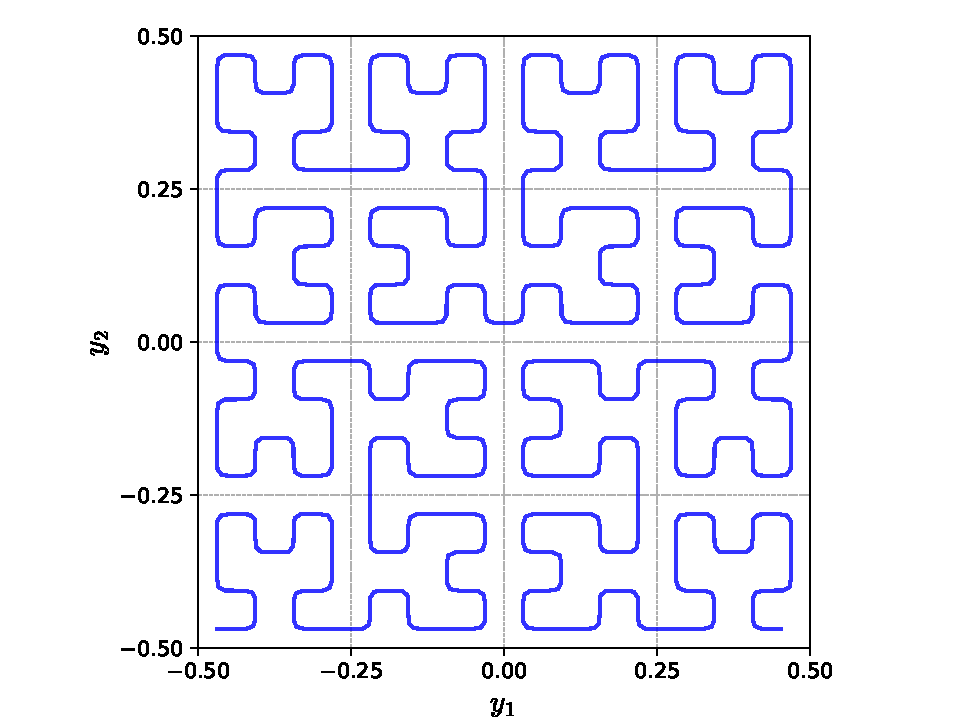
\includegraphics[width=.6\textwidth]{pictures/smooth.pdf}}\label{fig:smooth}}
    \subfloat[Non-univalent
evolvent]{{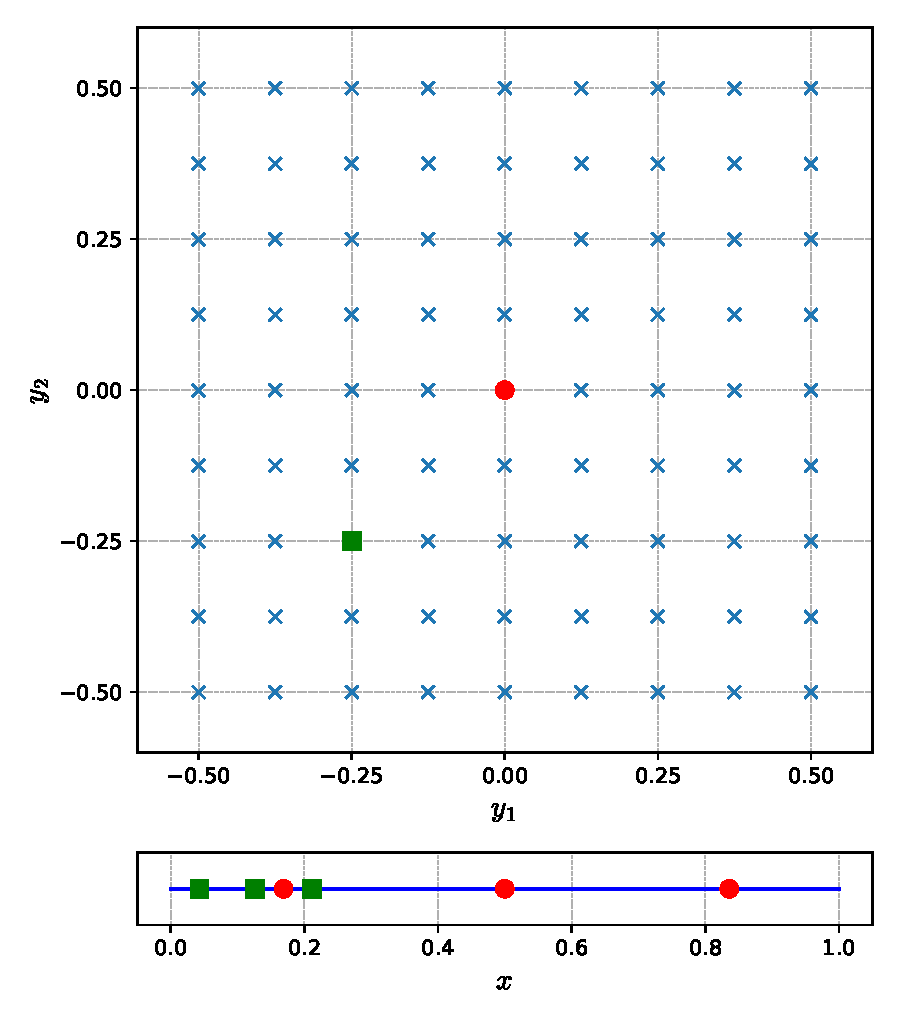
\includegraphics[width=.4\textwidth]{pictures/noninjective.pdf}}\label{fig:noninjective}}
    \caption{Different evolvents built with low density}
\end{figure}

\section{Parallel Computations for Solving Global Optimization Problems.}
\subsection{Core Multidimensional Algorithm of Global Search (MAGS)}

The optimization methods applied in Globalizer to solve the reduced problem
(\ref{eq:oneDimTask}) are based on the MAGS method, which can be presented as follows ---
see \cite{strongin1978}, \cite{strSergGO}.
\par
The initial iteration of the algorithm is performed at an arbitrary point \mbox{\(x^1\in(0,1)\)}.
Then, let us suppose that \(k\), \(k\ge 1\), optimization iterations have been completed already.
The selection of the trial point \(x^{k+1}\) for the next iteration is performed according to the
following rules.

\textit{Rule 1}. Renumber the points of the preceding trials by the lower indices in order of
increasing value of coordinates
$0=x_0<x_1<...<x_{k+1}=1$.

\textit{Rule 2}. Compute the characteristics \(R(i)\) for each interval \((x_{i-1},x_i),1\leq i\leq
k+1\).

\textit{Rule 4}. Determine the interval with the maximum characteristic $R(t)=\max_{1\leq i
\leq k+1}R(i)$.

\textit{Rule 5}. Execute a new trial at the point \(x^{k+1}\) located within the interval with the
maximum characteristic from the previous step
  $x^{k+1}=d(x_t)$.

The stopping condition, which terminated the trials, is defined by the inequality
$\rho_t<\varepsilon$
for the interval with the maximum characteristic from Step 4 and \(\varepsilon >0\) is the
predefined
accuracy of the optimization problem solution. If the stopping condition is not satisfied,
the index \(k\) is incremented by 1, and the new global optimization iteration is executed.

The convergence conditions and exact formulas for descision rules $R(i)$ and $d(x)$ of the
described algorithm are given, for example, in \cite{strSergGO}.

The numerical experiments, the results of which are presented in \cite{GergelLebedev,GergelSidorov} demonstrate that the method, at least, is not worse than the well-known global optimization algorithms DIRECT \cite{Jones} and DIRECT\textit{l} \cite{Gablonsky}, and even overcome these ones with respect to some parameters.

%------------------------------------------------------------------------------
\subsection{Parallel algorithm exploiting a set of evolvents}
\label{sec:parallel_evolvents}
Using the multiple mapping allows solving initial problem (\ref{eq:task}) by parallel solving the
problems
\[
\min\{\varphi(y^s(x)):x\in [0,1]\}, 1\leqslant s\leqslant S
\]
on a set of intervals $[0,1]$ by the index method. Each one-dimensional problem is solved on a
separate processor. The trial results at the point \(x^k\) obtained for the problem being solved by
particular processor are interpreted as the results of the trials in the rest problems (in the
corresponding points \(x^{k_1},\dots,x^{k_S})\). In this approach, a trial at the point \(x^k \in
[0,1]\) executed in the framework of the \(s\)-th problem, consists in the following sequence of
operations.
\par
1. Determine the image \(y^k=y^s (x^k)\) for the evolvent \(y^s (x)\).
\par
2. Inform the rest of processors about the start of the trial execution at the point \( y^k\) (the
blocking of the point \(y^k\) ).
\par
3. Determine the preimages \(x{}^{k_s}  \in [0,1], 1\leqslant s\leqslant S\), of the point \(y^k\) and interpret the
trial executed at the point \(y^k \in D \) as the execution of the trials in the \(S\) points
\(x{}^{k_1} ,\dots,x{}^{k_s} \)
\par
4. Inform the rest of processors about the trial results at the point \(y^k\).
\par

The decision rules for the proposed parallel algorithm, in general, are the same as the rules of the
sequential algorithm (except the method of the trial execution). Each processor has its own copy
of the software realizing the computations of the problem functions and the decision rule of the
index algorithm. For the organization of the interactions among the processors, the queues are
created on each processor, where the processors store the information on the executed iterations
in the form of the tuples: the processor number \(s\), the trial point \(x{}^{k_s}\).
\par
The proposed parallelization scheme was implemented with the use of MPI technology. Main
features of implementation consist in the following. A separate MPI-process is created for each
of \(S\) one-dimensional problems being solved, usually, one process per one processor
employed. Each process can use $p$ threads, usually one thread per an accessible core.
\par
At every iteration of the method, the process with the index \(s,0\leqslant s< S\) performs p
trials in parallel at the points \(x^{(s+iS)},0\leqslant i<p\). At that, each process stores all
\(S_p\) points, and an attribute indicating whether this point is blocked by another process or
not is stored for each point. Let us remind that the point is blocked if the process starts the
execution of a trial at this point.
\par
At every iteration of the algorithm, operating within the \(s\)-th process, determines the
coordinates of \(p\) ``its own" trial points. Then, the interchange of the coordinates of images of
the trial points \(y^{(s+iS)},0\leqslant i<p, 0\leqslant s< S\) is performed (from each process to
each one). After that, the preimages \(x^{(q+iS)},0\leqslant q<S,q\not=s\) of the points
received by the \(s\)-th process from the neighbor ones are determined with the use of the
evolvent \(y^s (x)\). The points blocked within the \(s\)-th process will correspond to the
preimages obtained. Then, each process performs the trials at the non-blocked points, the
computations are performed in parallel using OpenMP. The results of the executed trials (the
index of the point, the computed values of the problem functions, and the attribute of
unblocking of this point) are transferred to all rest processes. All the points are added to the
search information database, and the transition to the next iteration is performed.

%------------------------------------------------------------------------------
\section{Results of Numerical Experiments}
%\begin{Russian}

The computational experiments have been carried out on the Lobachevsky supercomputer at
State University of Nizhni Novgorod. A computational node included 2 Intel
Sandy Bridge E5-2660 2.2 GHz processors, 64 GB RAM. The CPUs had 8 cores (i. e. total 16
cores were available per a node). All considered algorithms and evolvents were implemented
using C++ within the Globalizer software system~\cite{globalizerSystem}.
In order to enable the parallelism,
OpenMP was used on a single node, and MPI was used for the parallelization on
several nodes.

The comparison of the global optimization algorithms was performed by the evaluation of the
quality of solving a set of problems from some test class.
In the present paper, the test class generated by GKLS (Gaviano, Kvasov, Lera, Sergeyev) generator~\cite{Gaviano2003} was
considered. The generator creates objective functions by distorting a convex quadratic function by polynomials in order to introduce local minima.
Thus, GKLS allows constructing the complex multiextremal problems of various dimensions.
In the present work, the series of 100 problems from the classes of the dimensions
of 2, 3, 4, and 5 were considered.
Each class had two degrees of complexity --- \textit{Simple} and \textit{Hard}. These the classes have different
radius of the attraction region of the global minimizer (\textit{Hard} has smaller region) and distance from the global minimizer to the vertex of the quadratic function (\textit{Simple} has smaller distance).
The parameters of the generator for the considered classes were given in Ref.~\cite{Gaviano2003}.

%\end{Russian}

In order to evaluate the efficiency of an algorithm on a given set of 100 problems, we will use
the operating characteristics \cite{grishaginClass}, which are defined as a
curve, showing the dependency of number of solved problems vs the number of iterations.

%------------------------------------------------------------------------------
\subsection{Comparison of the sequential evolvents}
\label{sec:seq_comp}
%\begin{Russian}
In order to understand whether any type of evolvents listed above has an essential advantage as
compared to other ones, the operating characteristics of the index method with different types
of evolvents have been obtained for the classes GKLS 2d Simple and GKLS 3d Simple. The
global minimum was considered to be found if the algorithm generates a trial point $y^k$ in the
$\delta$-vicinity of the global minimizer, i.e. $\left\|y^k-y^\ast\right\|_\infty\leq\delta$. The size
of the vicinity was selected as $\delta = 0.01\left\|b-a\right\|_\infty$. In case of GKLS
$\delta=0.01$.

In all experiments, the evolvent construction density parameter $m=12$. The minimum value of
the reliability parameter \(r\) was found for each type of evolvents by scanning over a uniform grid
with the step \(0.1\).

On the GKLS 2d Simple class at the minimum \(r\), the non-univalent evolvent and the smooth
one provide a faster convergence (Fig.~\ref{fig:gkls2d_opt}). The same was observed at
\(r=5.0\) as well (Fig.~\ref{fig:gkls2d_acc}). In the latter case, the shifted evolvent and the
rotating one begin to lag behind the rest since the value \(r=5.0\) is too big for them.
\begin{figure}[ht]
    \centering

\subfloat[$r=5.0$]{{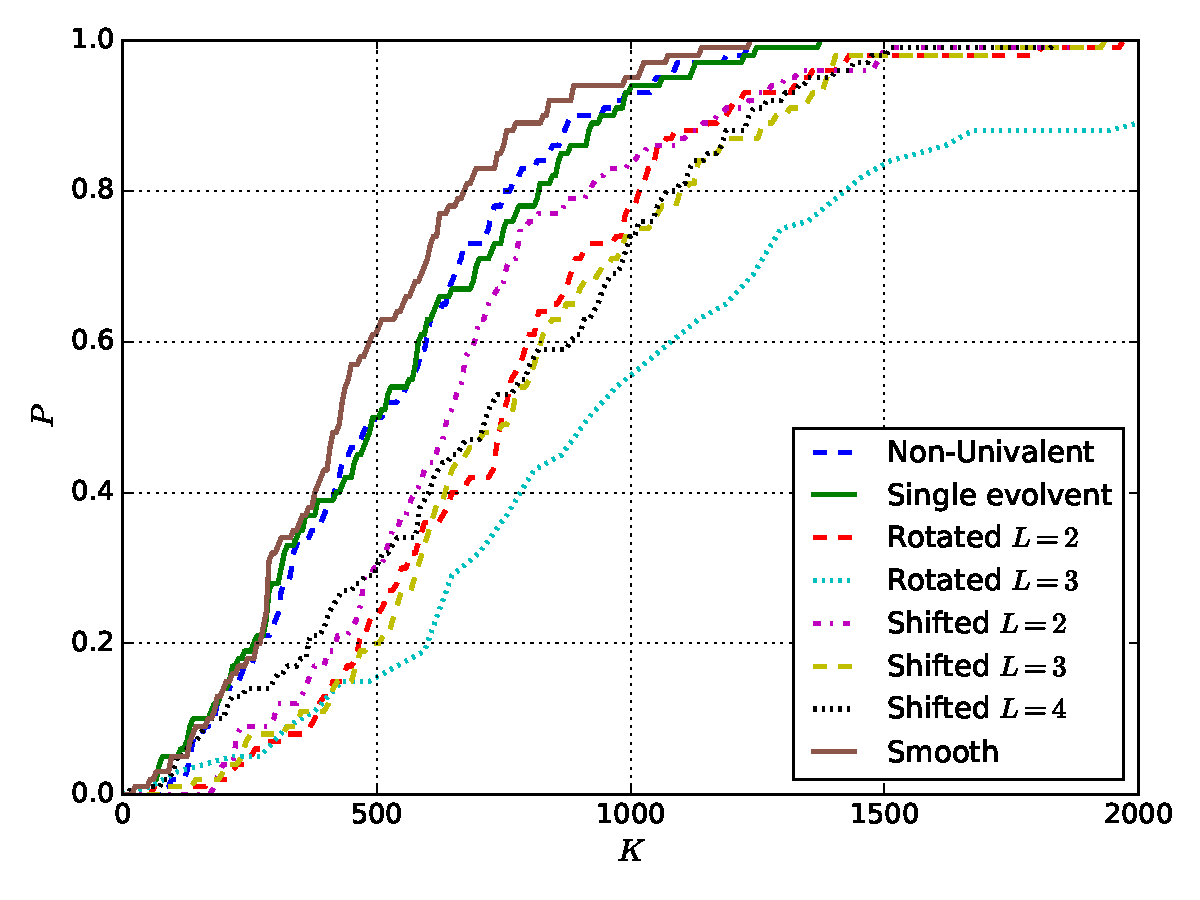
\includegraphics[width=.5\textwidth]{pictures/gklsS2d_same_r_opt_pt_op.pdf}}\label{fig:gkls2d_acc}}
    \subfloat[Minimal
$r$]{{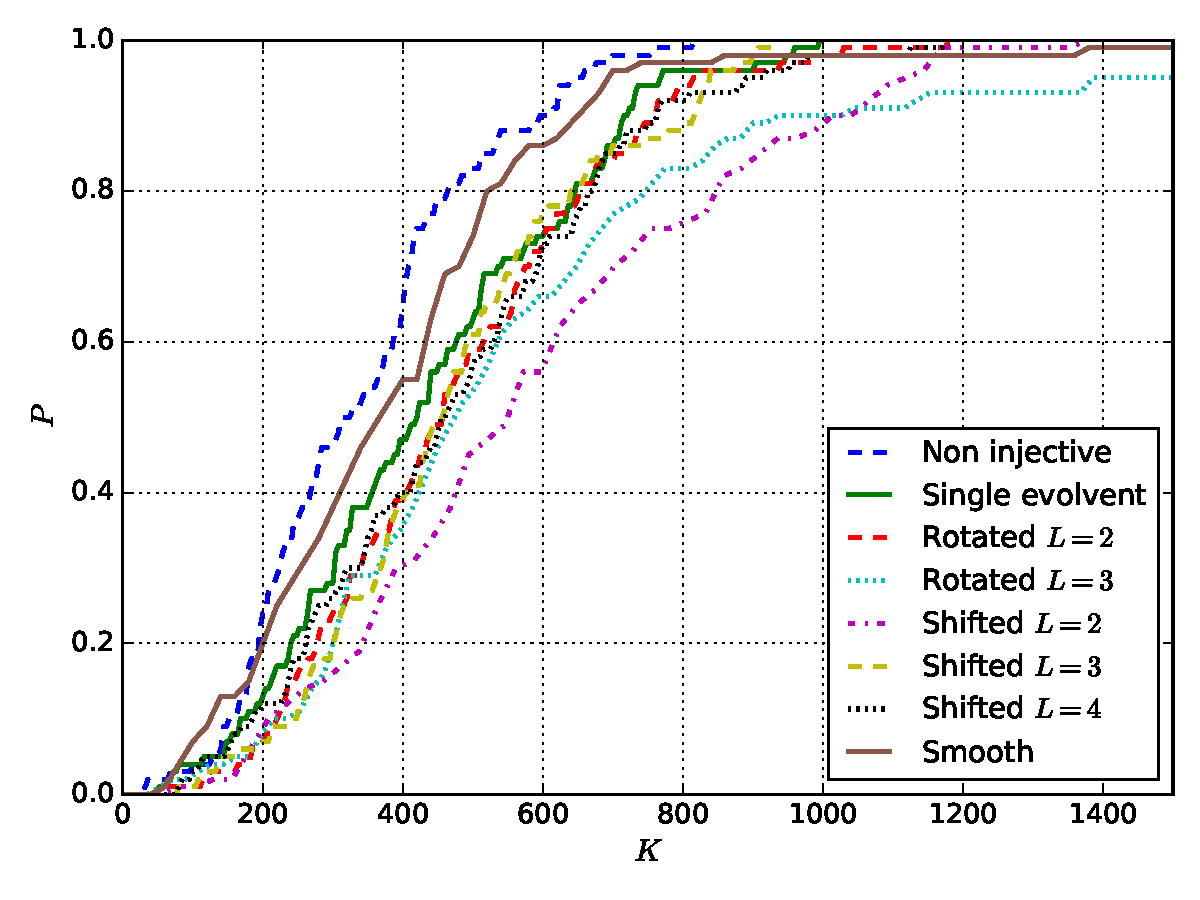
\includegraphics[width=.5\textwidth]{pictures/gklsS2d_opt_pt_op.pdf}}\label{fig:gkls2d_opt}}
    \caption{Operating characteristics on GKLS 2d Simple class}
\end{figure}

On the GKLS 2d Simple class at the minimum \(r\), the non-univalent evolvents and multiple
ones have a considerable advantage over the single evolvent (Fig.~\ref{fig:gkls3d_opt}).
The value \(r=4.5\) is too big for the rotated evolvents and for the shifted one
(Fig.~\ref{fig:gkls3d_acc}).

\begin{figure}[ht]
    \centering

\subfloat[$r=4.5$]{{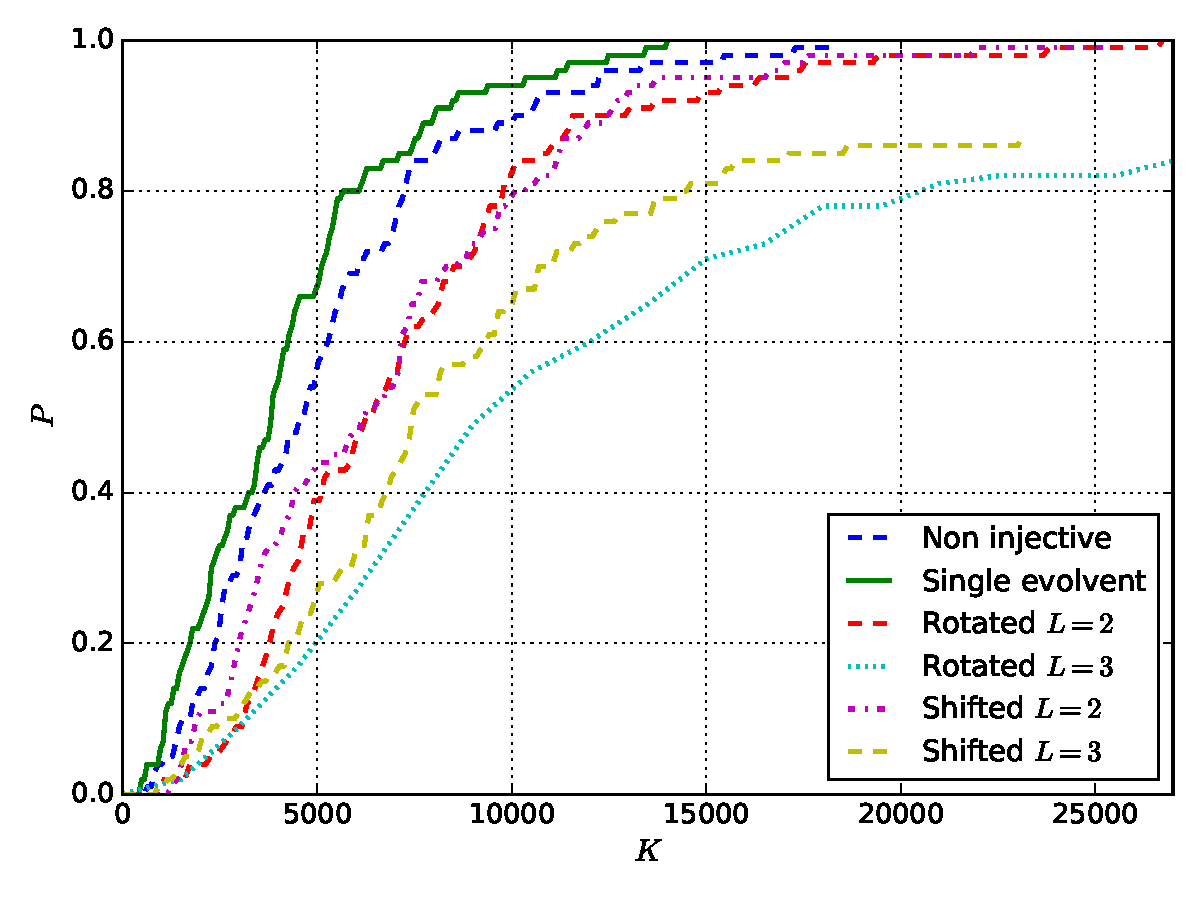
\includegraphics[width=.5\textwidth]{pictures/gklsS3d_same_r_opt_pt_op.pdf}}\label{fig:gkls3d_acc}}
    \subfloat[Minimal
$r$]{{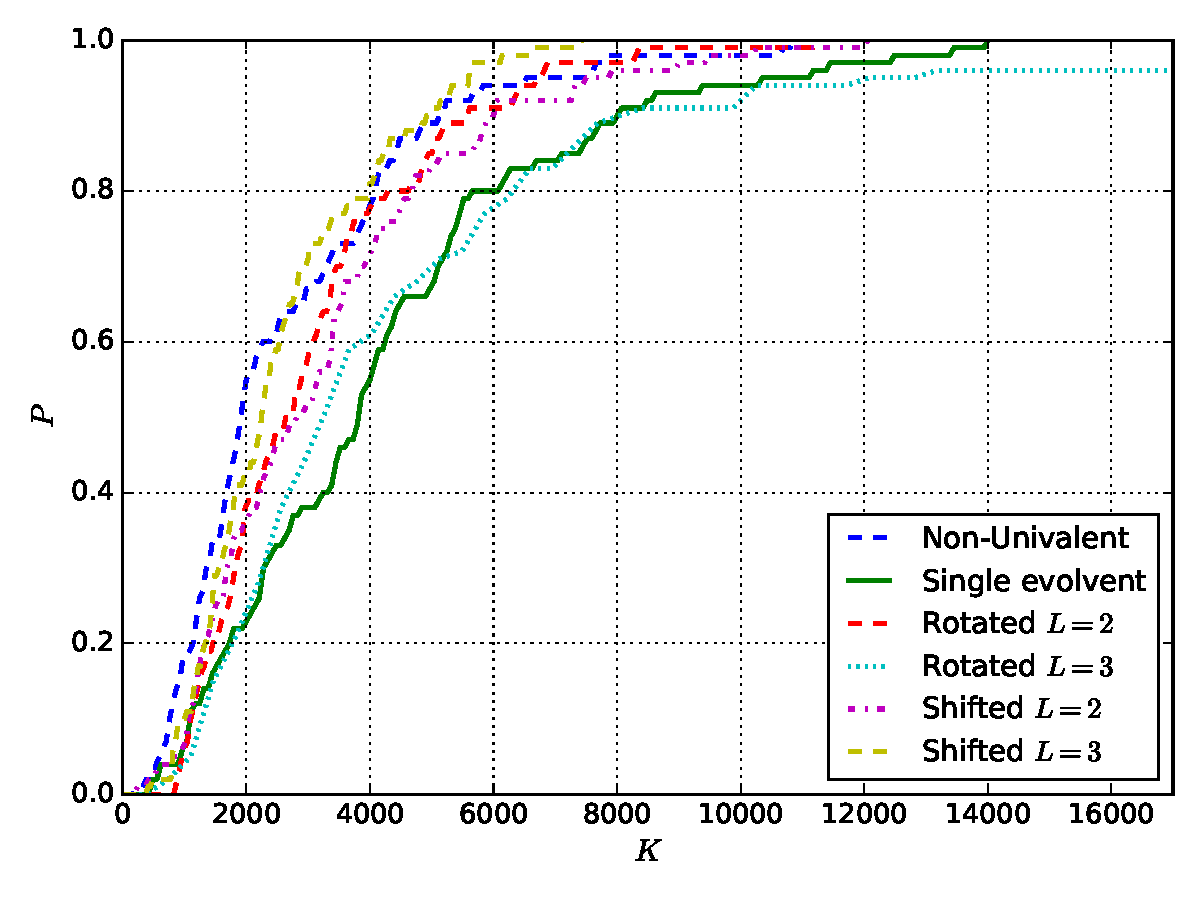
\includegraphics[width=.5\textwidth]{pictures/gklsS3d_opt_pt_op.pdf}}\label{fig:gkls3d_opt}}
    \caption{Operating characteristics on GKLS 3d Simple class}
\end{figure}

\paragraph{Overhead costs when using the shifted evolvents.}
In all experiments presented above, the number of computations of the objective function from
the GKLS class was taken into account when plotting the operating characteristics. However, in
the case of the shifted evolvent, the index method solves the problem with the constraint \(g_0\)
from (\ref{6_g0}). At the points where \(g_0\) is violated, the value of the objective function is
not computed. Nevertheless, these points are stored in the search information producing the
additional computational costs. In Table~\ref{tab:shifted_g0}, the averaged numbers of calls to
\(g_0\) and to the objective function are presented. At \(L=3\), the constraint \(g_0\) was
computed almost 20 times more than the objective function \(\varphi\) i. e. \(95\%\) of the whole
search information account for the auxiliary points. Such overhead costs are acceptable when
solving the problems of small dimension with the computation costly objective functions.
However, when increasing dimensionality and total number of trials other types of evolvents are
preferred.

\begin{table}
\begin{center}
\caption{Averaged number of computations of \(g_0\) and of \(\varphi\) when solving the
problems from GKLS 3d Simple class using the shifted evolvent}
  \begin{tabular}{|l|{c}|{c}|{c}|}
    \hline
  $L$ & $calc(g_0)$ & $calc(\varphi)$ & $\frac{calc(g_0)}{calc(\varphi)}$ ratio \\
  \hline
  2 & 96247.9  & 6840.14 & 14.07\\
  \hline
  3 & 153131.0 & 7702.82 & 19.88\\
  \hline
  \end{tabular}
  \label{tab:shifted_g0}
\end{center}
\end{table}

%------------------------------------------------------------------------------
\subsection{Parallel rotated evolvents}
\label{sec:results_parallel}
In order to evaluate the efficiency of the parallel algorithm from
Sec.~\ref{sec:parallel_evolvents}, the numerical experiments on the GKLS 4d (Hard, Simple)
classes and on the GKLS 5d (Hard, Simple) ones were conducted. The value of \(r\) in all
experiments was equal to 5.0, the size of the \(\delta\)-vicinity of the known solution was
increased up to 0.3. When solving the series of problems, up to 8 cluster nodes and up to 32
computational threads on each node were employed.

In Table~\ref{tab:iterations}, an averaged number of iterations when solving 100 problems from
each considered class is presented.
The number of iterations is reduced considerably with increasing the number of nodes and the
number of threads on each node (except the GKLS 4d Simple class at the transition from 1
node to 4 ones in the single thread mode).

\begin{table}
  \centering
  \caption{Averaged numbers of iterations executed by the parallel algorithm for solving the test
optimization problems}
  \label{tab:iterations}
  \begin{tabular}{cccccccc}
    \cline{3-8}\noalign{\smallskip}
    \multicolumn{2}{c}{  } & \textit{p} & \multicolumn{2}{c}{$N=4$} & &
\multicolumn{2}{c}{$N=5$}   \\
    \noalign{\smallskip} \cline{4-5} \cline{7-8}  \noalign{\smallskip}
    \multicolumn{2}{c}{  } & & \textit{Simple} & \textit{Hard} & & \textit{Simple} &
\textit{Hard}  \\
    \noalign{\smallskip}\hline
    I &
    \parbox{0.25\textwidth}{
    \begin{center}
    \textbf{1 cluster node}
    \end{center}		}
      & \textit{1} & 12167 & 25635 & & 20979 & 187353  \\
    &  & \textit{32} & 328 & 1268  & &   898 & 12208 \\
    \hline \noalign{\smallskip}
II  & \textbf{4 cluster nodes}  %\multirow{3}{*}{}
  & \textit{1} & 25312 & 11103 & & 1472 & 17009 \\
&   & \textit{32} & 64 &   913 & & 47 & 345 \\
    \noalign{\smallskip}\hline	\noalign{\smallskip}
III & \textbf{8 cluster nodes} %\multirow{3}{*}{}
  & \textit{1}  & 810 & 4351 & & 868 & 5697  \\
& & \textit{32} & 34  & 112  & & 35  & 868 \\
    \noalign{\smallskip}\hline
  \end{tabular}
\end{table}

If one assumes the costs of parallelization to be negligible as compared to the costs of
computing the objective functions in the optimization problems, the speedup in time due to the
use of the parallel method would be equal to the speedup with respect to the number of
iterations. However, actually this suggestion is not always true. In all numerical experiment the
time of computing the objective function was approximately $10^{-3}$ sec. In
Table~\ref{tab:speedup}, the speedups in iterations and in time (in the pendent brackets) are
presented. In the first row of the table corresponding to the sequential mode, the averaged time
of solving a single problem is presented in the pendent brackets. One can see from the table that
for the GKLS 4d classes it is more efficient to utilize a single node in the multithread mode
whereas for solving more complex five-dimensional problems, the use of several nodes is better,
each node is operating in the parallel mode.

\begin{table}
  \centering
  \caption{Speedup of parallel computations executed by the parallel algorithm}
  \label{tab:speedup}
  \begin{tabular}{cccccccc}
    \cline{3-8}\noalign{\smallskip}
    \multicolumn{2}{c}{  } & \textit{p} & \multicolumn{2}{c}{$N=4$} & &
\multicolumn{2}{c}{$N=5$}   \\
    \noalign{\smallskip} \cline{4-5} \cline{7-8}  \noalign{\smallskip}
    \multicolumn{2}{c}{  } & & \textit{Simple} & \textit{Hard} & & \textit{Simple} &
\textit{Hard}  \\
    \noalign{\smallskip}\hline
    I &
    \parbox{0.25\textwidth}{
    \begin{center}
    \textbf{1 cluster node}
    \end{center}		}
    & \textit{1}   & 12167(10.58s) & 25635(22.26s) & & 20979(22.78s) & 187353(205.83s)  \\
  &  & \textit{32} & 37.1(18.03) & 20.2(8.55)  & &  23.3(8.77) & 15.4(9.68) \\
  \hline \noalign{\smallskip}
II  & \textbf{4 cluster nodes}  %\multirow{3}{*}{}
& \textit{1} &        0.5(0.33) & 2.3(0.86)  & & 14.3(6.61) & 11.0(6.06) \\
&   & \textit{32} & 190.1(9.59) & 28.1(1.08) & & 446.4(19.79) & 543.0(43.60) \\
  \noalign{\smallskip}\hline	\noalign{\smallskip}
III & \textbf{8 cluster nodes} %\multirow{3}{*}{}
& \textit{1}    & 15.0(6.05)  & 5.9(2.36)   & & 24.2(17.56)  & 32.9(24.87)  \\
& & \textit{32} & 357.9(2.36) & 228.9(2.64) & & 582.8(20.96) & 793.0(33.89) \\
    \noalign{\smallskip}\hline
  \end{tabular}
\end{table}

%------------------------------------------------------------------------------
\section{Conclusions}
In the present work, 5 different Peano curve-type mappings applied to the dimensionality
reduction in the global optimization problems were considered.
From the preliminary comparison conducted in Sec.~\ref{sec:seq_comp}, one can make the
following conclusions:
\begin{itemize}
  \item the smooth evolvent and the non-univalent one demonstrate the best result in the
problems of small dimensionality and can be applied successfully in solving the problems with
the computational costly objective functions. The properties of these evolvents don't allow
developing the optimization algorithms scalable onto several cluster nodes based on these ones.
  \item the shifted evolvents introduce large overhead costs on the operation of the method due
to the requirement to adding an auxiliary functional constraint into the problem (\ref{eq:task}).
The experiments have demonstrated that up to 95\% of the search information account for the
points, in which the auxiliary constraint is computed only. The shifted evolvents can be used as
the base for the parallel algorithm from Sec.~\ref{sec:parallel_evolvents}. However, the costs of
processing the auxiliary points would result likely in a small speedup from the parallelization.
However, if the objective function is computation-costly enough, the use of these evolvents
could make sense.
  \item the rotated evolvents have provided an acceptable speed of convergence in the problems
of small dimensionality in the sequential mode. The use of these ones don't result in the
introduction of the auxiliary constraints that allows constructing an efficient parallel algorithm
based on these evolvents.
\end{itemize}

In Sec.~\ref{sec:results_parallel} the results of the numerical experiments are presented, which
have demonstrated the algorithm from Sec.~\ref{sec:parallel_evolvents} based on the rotated
evolvents allowed obtaining the speedup up to 43 times when solving the problem series
employing several nodes of the computer cluster. It is worth noting that the objective functions
in the considered problems are not computation-costly (the averaged computation time was
$10^{-3}$ sec). In the case of more complex problems,the speedup in time could approach the
speedup with respect to the number of iterations.
%\end{Russian}

% ---- Bibliography ----
%
% BibTeX users should specify bibliography style 'splncs04'.
% References will then be sorted and formatted in the correct style.
%
% \bibliographystyle{splncs04}
% \bibliography{mybibliography}
%
\begin{thebibliography}{107}

\bibitem{sergeyevStronginLera2013}% (MR3113120) [10.1007/978-1-4614-8042-6]
\newblock Y. D. Sergeyev, R. G. Strongin and D. Lera,
\newblock \emph{Introduction to Global Optimization Exploiting Space-filling Curves},
\newblock Springer (2013)

\bibitem{strongin1978}% (MR509033)
\newblock R. G. Strongin,
\newblock \emph{Numerical Methods in Multi-Extremal Problems (Information-Statistical Algorithms)},
\newblock Moscow: Nauka (1978) (In Russian)

\bibitem{Strongin1992}% (MR1263606) [10.1007/BF00122428]
\newblock R. G. Strongin,
\newblock \emph{\emph{Algorithms for multi-extremal mathematical programming problems
employing a set of joint space-filling curves}},
\newblock \emph{J. Glob. Optim.}, \textbf{2}, 357--378 (1992)

\bibitem{stronginGergelBarkalovParGO}
\newblock R. G. Strongin, V. P. Gergel, V. A. Grishagin and K. A. Barkalov,
\newblock \emph{Parallel Computations for Global Optimization Problems},
\newblock Moscow State University, Moscow (2013) (In Russian)

\bibitem{strSergGO}%5 (MR1797058) [10.1007/978-1-4615-4677-1]
\newblock R. G. Strongin and Y. D. Sergeyev,
\newblock \emph{Global Optimization with Non-convex Constraints. Sequential and Parallel
Algorithms},
\newblock Kluwer Academic Publishers, Dordrecht (2000, 2nd ed. 2013, 3rd ed. 2014)

\bibitem{zilinskTornGO}% (MR1100586) [10.1007/3-540-50871-6]
\newblock A. T\"orn and A. \v Zilinskas,
\newblock \emph{Global Optimization},
\newblock Springer, (1989)

\bibitem{Goryachih2017}
\newblock Goryachih, A.
\newblock \emph{A class of smooth modification of space-filling curves for global optimization
problems}
\newblock Springer Proceedings in Mathematics and Statistics, \textbf{197}, pp. 57--65 (2017)

\bibitem{zhigljavskyRandGO}% (MR1187048) [10.1007/978-94-011-3436-1]
\newblock A. A. Zhigljavsky,
\newblock \emph{Theory of Global Random Search},
\newblock Kluwer Academic Publishers, Dordrecht (1991)

\bibitem{Strongin1991}
Strongin, R.G.: \emph{Parallel multi-extremal optimization using a set of evolvents}. Comp. Math.
Math. Phys. \textbf{31(8)}, 37--46 (1991)

\bibitem{Gergel2009}
Strongin, R.G., Gergel, V.P., Barkalov, K.A.: \emph{Parallel methods for global optimization problem
solving.} Journal of instrument engineering. \textbf{52}, 25--33 (2009) (In Russian)

\bibitem{Gaviano2003}
Gaviano, M., Kvasov, D.E, Lera, D., and Sergeyev, Ya.D.: \emph{Software for generation of classes
of test functions with known local and global minima for global optimization.} ACM
Transactions on Mathematical Software \textbf{29(4)}, 469--480 (2003)

\bibitem{grishaginClass}
Grishagin, V.A.: \emph{Operating Characteristics of Some Global Search Algorithms.} Problems of
Statistical Optimization \textbf{7}, 198--206 (1978) (In Russian)

\bibitem{globalizerSystem}
Gergel V.P., Barkalov K.A., and Sysoyev A.V: Globalizer: \emph{A novel supercomputer software
system for solving time-consuming global optimization problems.} Numerical Algebra, Control
\& Optimization \textbf{8(1)}, 47--62 (2018)

%\bibitem{Sergeyev2006}
%Sergeyev, Ya.D., Kvasov, D.E.: \emph{Global search based on efficient diagonal partitions and a set
%of Lipschitz constants}. SIAM J. Optim \textbf{16(3)}, 910--937 (2006)

\bibitem{SergeyevKvasov2015}
Sergeyev, Y.D., Kvasov, D.E.: \emph{A deterministic global optimization using smooth diagonal
auxiliary functions.} Communications in Nonlinear Science and Numerical Simulation. \textbf{21(1-3)},
99--111 (2015)

%\bibitem{Zilinskas2008}
%\v Zilinskas, J.: \emph{Branch and bound with simplicial partitions for global optimization.} Math.
%Model. Anal. \textbf{13(1)}, 145--159 (2008)

\bibitem{Zilinskas2014}
Paulavi\v cius, R., \v Zilinskas, J.: \emph{Simplicial Lipschitz optimization without the Lipschitz
constant.} J. Glob. Optim. \textbf{59(1)}, 23--40 (2014)

\bibitem{Jones}
Jones, D.R.: The direct global optimization algorithm. In: Floudas, C.A., Pardalos, P.M.
(eds.) \emph{The Encyclopedia of Optimization}, 2nd edn., pp. 725--735. Springer, Heidelberg
(2009)

\bibitem{Gablonsky}
Gablonsky, J.M., Kelley, C.T.: \emph{A locally-biased form of the DIRECT algorithm.} J. Glob.
Optim., \textbf{21(1)}, 27--37 (2001)

\bibitem{Evtushenko}
Evtushenko, Y., Posypkin, M.: \emph{A deterministic approach to global box-constrained
optimization.} Optim. Lett. \textbf{7(4)}, 819--829 (2013)

\bibitem{GergelLebedev}
Gergel V. and Lebedev I. \emph{Heterogeneous Parallel Computations for Solving Global Optimization Problems.} Proc. Comput. Science \textbf{66}, pp. 53--62 (2015)

\bibitem{GergelSidorov}
Gergel V., Sidorov S. \emph{A Two-Level Parallel Global Search Algorithm for Solution of Computationally Intensive Multiextremal Optimization Problems.} {Lect. Notes Comput. Science} \textbf{9251}, pp. 505--515 (2015)

\end{thebibliography}
\end{document}
